\documentclass{standalone}
\usepackage{tikz}

\begin{document}

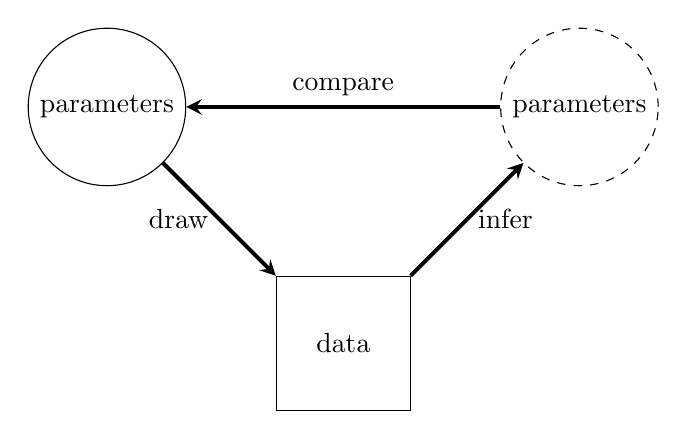
\begin{tikzpicture}
    \tikzset{common size/.style={minimum size=2cm, align=center}}
    \node[draw, circle, common size] (circle1) at (0,0) {parameters};
    \node[draw, dashed, circle, common size] (circle2) at (6,0) {parameters};
    \node[draw, rectangle, minimum size = 1.7cm] (box) at (3,-3) {data};
    \draw[->, thick, >=stealth, line width=0.5mm] (circle1) -- (box) node[midway, left] {draw};
    \draw[->, thick, >=stealth, line width=0.5mm] (box) -- (circle2) node[midway, right] {infer};
    \draw[->, thick, >=stealth, line width=0.5mm] (circle2) -- (circle1) node[midway, above] {compare};
\end{tikzpicture}

\end{document}